%instiki:category: QuantumFieldTheory
\chapter{Feynman Rules}
\label{chap:fr} %noinstiki
%instiki:
%instiki:***
%instiki:
%instiki:[[Beyond|Contents]]
%instiki:
%instiki:***
%instiki:
%instiki:* [Interaction picture](#interaction-picture)
%instiki:
%instiki:* [Yukawa interaction](#feynman-diagrams)
%instiki:
%instiki:* [Scattering](#scattering)
%instiki:

When the case of interacting fields are considered, the particles can be created, destroyed and scattered. In essence this requires solving the coupled non-linear field equations for given conditions. This is an extremely difficult problem which has only been solved in perturbation theory.

In the Heisenberg picture, which we have so far been using, this program is still very complex, and it was decisive for the successful development of the theory to work instead in the interaction picture. In section \ref{sec:interaction-picture} we write the $S$--matrix expansion derived in Chapter~\ref{cha:s-matrix}, in the interaction picture. In section \ref{sec:feynman-diagrams} we show how to use the Wick expansion to calculate $S$--matrix elements involving scalars and spinors.

\section{Interaction picture}
\label{sec:interaction-picture}
This part is based in \cite{Mandl:1985bg}. 
In the Schr\"odinger Picture (SP) the time dependence is carried by the states according to the Scr\"odinger equation 
\begin{align}
\label{eq:84}
  i\frac{\partial}{\partial t}|a,t\rangle_{\text{S}}=  i\frac{d}{dt}|a,t\rangle_{\text{S}}=  {H}|a,t\rangle_{\text{S}}
\end{align}
With the solution given in Eq.~\eqref{eq:39}
\begin{align}
\label{eq:85}
    |a,t\rangle_{\text{S}}=U(t,t_i)|a\rangle_{\text{S}}\,.
\end{align}
where $U$ is the unitary operator [see Eq.~\eqref{eq:40}]
\begin{align}
 U\equiv U(t,t_i)= e^{-i H(t-t_i)}\,.
\end{align}
Given the state $|a,t\rangle_{\text{S}}$ in the SP, in the Heisenberg picture (HP) we defined the state
\begin{align}
\label{eq:86}
  |a\rangle_H=U^\dagger|a,t\rangle_{\text{S}}=|a\rangle_{\text{S}}
\end{align}
Si $O^{\text{S}}$ in an operator in the SP, the corresponding Heisenberg operator is defined as
\begin{align}
\label{eq:87}
  O^{\text{H}}(t)=U^\dagger O^{\text{S}}U
\end{align}
Hence, the transformation from HP to SP is unitary. At $t=t_i$, states and operators in the two pictures are the same. We see from Eq.~\eqref{eq:86} that in the HP state vectors are constant in time, while from Eq.~\eqref{eq:87} the Heisenberg operators evolve with time. Is convenient to keep the temporal label in the Heisenberg states
\begin{align}
  |a\rangle_H=|a,t_i\rangle_H
\end{align}
Eq.~\eqref{eq:87} ensures the invariance of matrix elements and commutation relations:
\begin{align}
  {}_{\text{S}}\langle b,t|\,O^{\text{S}}\,|a,t\rangle_{\text{S}}=  {}_{\text{S}}\langle b,t|\,U O^{\text{H}}(t) U^\dagger\,|a,t\rangle_{\text{S}}=
{}_{\text{H}}\langle b,t_i|O^{\text{H}}(t)|a,t_i\rangle_{\text{H}}
\end{align}
\begin{align}
\left[O^{\text{S}},P^{\text{S}}\right]=c\Rightarrow\left[O^{\text{H}}(t),P^{\text{H}}(t)\right]=c
\end{align}
where $c$ is a constant.

Differentiation of Eq. \eqref{eq:87} 
\begin{align}
  \frac{d}{dt}O^{\text{H}}(t)=&\left(\frac{d}{dt}U^\dagger\right)O^{\text{S}}U+
U^\dagger O^{\text{S}}\frac{d}{dt}U\nonumber\\
 =&i H\, U^\dagger O^{\text{S}}U+
U^\dagger O^{\text{S}}U(-i H)\nonumber\\
 =&-i ( O^{\text{H}}H-H O^{\text{H}})\,,
\end{align}
gives the Heisenberg equation of motion

\begin{align}
  i\frac{d}{dt}O^{\text{H}}(t)=\left[O^{\text{H}}(t),H\right]
\end{align}
The interaction picture (IP) arises if the Hamiltonian is split into two parts
\begin{align}
  H=H_0+H_{\text{I}}\,.
\end{align}
In quantum field theory $H_I$ will describe the interaction between two fields, themselves described by $H_0$

IP is related to the SP by the unitary transformation
\begin{align}
\label{eq:88}
  U_i\equiv U_i(t,t_i)=e^{-i H_i(t-t_i)}\,,
\end{align}
in this way,
\begin{align}
\label{eq:89}
  |a,t\rangle_{\text{I}}=U_0^\dagger|a,t\rangle_{\text{S}}\,,
\end{align}
and
\begin{align}
\label{eq:90}
  O^{\text{I}}(t)=U^\dagger_0 O^{\text{S}}U_0\,.
\end{align}
Thus the relation between IP and SP is similar to that between HP and SP, but with the unitary transformation $U_0$ involving only the non--interacting Hamiltonian $H_0$. Note that both the vector states as the operators in the IP are time-dependent.

Differentiating Eq.~\eqref{eq:90} gives the differential equation of motion operators in the IP:
\begin{align}
  i\frac{d}{dt}O^{\text{I}}(t)=\left[O^{\text{I}}(t),H_0\right]
\end{align}

Substituting Eq.~\eqref{eq:89} into the Scr\"odinger Eq.~\eqref{eq:84}, one obtains the equation of motion of state vectors in the IP, If the system is described by a time-dependent state vector $|\Phi(t)\rangle$
\begin{align}
  i\frac{d}{dt}|a,t\rangle_{\text{S}}=&  H^{\text{S}}|a,t\rangle_{\text{S}}\nonumber\\
  i\frac{d}{dt}\left(U_0|\Phi(t)\rangle\right)=&  H^{\text{S}}U_0|\Phi(t)\rangle\nonumber\\
  i\left(\frac{d}{dt}U_0\right)|\Phi(t)\rangle+iU_0\frac{d}{dt}|\Phi(t)\rangle=&  H^{\text{S}}U_0|\Phi(t)\rangle\nonumber\\
  U_0 H_0|\Phi(t)\rangle+iU_0\frac{d}{dt}|\Phi(t)\rangle=&  H^{\text{S}}U_0|\Phi(t)\rangle\nonumber\\
  U_0 H_0|\Phi(t)\rangle+iU_0\frac{d}{dt}|\Phi(t)\rangle=&  (H_0+H_I^{\text{S}})U_0|\Phi(t)\rangle\nonumber\\
  iU_0\frac{d}{dt}|\Phi(t)\rangle=&  H_I^{\text{S}}U_0|\Phi(t)\rangle\nonumber\\
  i\frac{d}{dt}|\Phi(t)\rangle=& U_0 H_I^{\text{S}}U_0|\Phi(t)\rangle
\end{align}
\begin{align}
\label{eq:91}
  i\frac{d}{d t}|\Phi(t)\rangle_{\text{I}}=H^{\text{I}}_I\,|\Phi(t)\rangle_{\text{I}}\,,
\end{align}
where, as in Eq.~\eqref{eq:90}
\begin{align}
  \label{eq:92}
  H^{\text{I}}_I=e^{i H_0^{{\text{S}}}(t-t_i)}H^{\text{S}}_I e^{-i H_0^{{\text{S}}}(t-t_i)}
\end{align}
is the interaction Hamiltonian in the IP, with $H^{\text{S}}_I$ and $H^{\text{S}}_0$ being the interaction and free-field Hamiltonian in the SP. From now on we shall omit the labels I, used in the equations to distinguish the IP, as we shall be working exclusively in the IP in what follows.

Eq. \eqref{eq:91} is a Scr\"odinger-like equation with the time dependent Hamiltonian $H_I(t)$. With the interaction switched off (i.e.  we put $H_I=0$), the state vector is constant in time. The interaction leads to the state $|\Phi(t)\rangle$ changing with time. Given that the system is in a state  $|i\rangle$ at an initial time $t=t_i$, i.e.
\begin{align}
\label{eq:93}
  |\Phi(t_i)\rangle=|i\rangle\,,
\end{align}
the solution of Eq.~\eqref{eq:91} with this initial condition gives the state $|\Phi(t)\rangle$ of the system at any other time $t$. It follows from the Hermicity of the operator $H_I(t)$ that the time development of the state $|\Phi(t)\rangle$ according to Eq.~\eqref{eq:91} is a unitary transformation. Accordingly it preserves the normalization of states
\begin{align}
  \langle\Phi(t)|\Phi(t)\rangle=\text{const}.
\end{align}
and, more generally, the scalar product.

Clearly the formalism which we are here developing is not appropriate for the description of bound states but it is particularly suitable for scattering processes. In a collision processes the state vector $|i\rangle$ will define an initial state, long before the scattering occurs ($t_i=-\infty$), by specifying a definite number of particles, with definite properties and far apart from each other so that they do not interact. (For example $|i\rangle$ would specify a definite number of electrons, and positrons with given momenta and spins). In the scattering process, the particles will come close together, collide (i.e interact) and fly apart gain. Eq.~\eqref{eq:91} determines the state $|\Phi(t)\rangle$ into which the initial state
\begin{align}
  |\Phi(-\infty)\rangle=|i\rangle\,,
\end{align}
evolves at $t=\infty$, long after the scattering is over and all particles are for apart again. The $S$--matrix relates $|\Phi(\infty)\rangle$ to $\Phi(-\infty)$ and is defined by
\begin{align}
  |\Phi(\infty)\rangle=S|\Phi(-\infty)\rangle=S|i\rangle\,,
\end{align}

A collision can lead to many different final states $|f\rangle$, and all these possibilities are constrained within $|\Phi(\infty)\rangle$.

The transition probability is given by
\begin{align}
  \left|\langle f|\Phi(\infty)\rangle\right|^2=  \left|\langle f|S|i\rangle\right|^2\equiv S_{f i}^2\,,
\end{align}
where $S_{f i}$ is the corresponding probability amplitude.

In order to calculate the $S$--matrix we must solve Eq.~\eqref{eq:91} for the initial condition \eqref{eq:93}. These equations can be combined into the integral equation
\begin{align}
 d |\Phi(t)\rangle=&-i d t\,H_I(t)|\Phi(t)\rangle\nonumber\\
\int_{|\Phi(-\infty)\rangle}^{|\Phi(t)\rangle} d |\Phi(t)\rangle=&-i \int_\infty^t d t_1\,H_I(t_1)|\Phi(t_1)\rangle\nonumber\\
|\Phi(t)\rangle-|\Phi(-\infty)\rangle=&-i \int_\infty^t d t_1\,H_I(t_1)|\Phi(t_1)\rangle\nonumber\\
\end{align}

\begin{align}
\label{eq:94}
  |\Phi(t)\rangle=|i\rangle-i\int_{-\infty}^t d t_1\,H_I(t_1)|\Phi(t_1)\rangle\,.
\end{align}
In the limit $t\to\infty$
\begin{align}
  |\Phi(\infty)\rangle=S^{(0)}|i\rangle-i\int_{-\infty}^\infty d t_1\,H_I(t_1)|\Phi(t_1)\rangle\,.
\end{align}
where 
\begin{align}
  S^{(0)}=1\,.
\end{align}
From Eq.~\eqref{eq:94} we can obtain $|\Phi(t_1)\rangle$ at next order:
\begin{align}
  |\Phi(t_1)\rangle=&|i\rangle-i\int_{-\infty}^{t_1} d t_2\,H_I(t_2)|\Phi(t_2)\rangle\,.
\end{align}


This equation then can  be solved iteratively. If $H_I$ is small we can solve this equation by iteration
\begin{align}
\label{eq:95}
  |\Phi(t)\rangle=|i\rangle+(-i)\int_{-\infty}^t d t_1 H_I(t_1)|i\rangle+(-i)^2\int_{-\infty}^t d t_1\int_{-\infty}^{t_1} d t_2\,H_I(t_1)H_I(t_2)|\Phi(t_2)\rangle\,.
\end{align}
In the limit $t\to\infty$
\begin{align}
  |\Phi(t)\rangle=&\left[S^{(0)}+(-i)\int_{-\infty}^\infty d t_1 H_I(t_1)\right]|i\rangle+(-i)^2\int_{-\infty}^\infty d t_1\int_{-\infty}^{t_1} d t_2\,H_I(t_1)H_I(t_2)|\Phi(t_2)\rangle\nonumber\\
  =&\left(S^{(0)}+S^{(1)}\right)|i\rangle+(-i)^2\int_{-\infty}^\infty d t_1\int_{-\infty}^{t_1} d t_2\,H_I(t_1)H_I(t_2)|\Phi(t_2)\rangle\,,
\end{align}
where 
\begin{align}
  S^{(1)}=(-i)\int_{-\infty}^\infty d t_1 H_I(t_1)\,.
\end{align}
The next order of Eq.~\eqref{eq:95} is
\begin{align}
  |\Phi(t)\rangle=&|i\rangle+(-i)\int_{-\infty}^t d t_1 H_I(t_1)|i\rangle+(-i)^2\int_{-\infty}^t d t_1\int_{-\infty}^{t_1} d t_2\,H_I(t_1)H_I(t_2)\nonumber\\
  &\times\left[|i\rangle+(-i)\int_{-\infty}^{t_2} d t_3 H_I(t_3)|i\rangle+(-i)^2\int_{-\infty}^{t_2} d t_3\int_{-\infty}^{t_3} d t_4\,H_I(t_3)H_I(t_4)|\Phi(t_4)\rangle\right]
\end{align}
\begin{align}
  |\Phi(t)\rangle=&|i\rangle+(-i)\int_{-\infty}^t d t_1 H_1(t_1)|i\rangle+(-i)^2\int_{-\infty}^t d t_1\int_{-\infty}^{t_1} d t_2\,H_I(t_1)H_I(t_2)|i\rangle\nonumber\\
  &+(-i)^3\int_{-\infty}^t d t_1\int_{-\infty}^{t_1} d t_2\int_{-\infty}^{t_2} d t_3\,H_I(t_1)H_I(t_2) H_1(t_3)|i\rangle\nonumber\\
  &+(-i)^4\int_{-\infty}^t d t_1\int_{-\infty}^{t_1}d t_2 \int_{-\infty}^{t_2} d t_3\int_{-\infty}^{t_3}d t_4 \,H_I(t_1)H_I(t_2)\,H_I(t_3)H_I(t_4)|\Phi(t_4)\rangle
\end{align}
In the limit $t\to\infty$
\begin{align}
  |\Phi(t)\rangle=&\left(S^{(0)}+S^{(1)}+S^{(2)}+S^{(3)}\right)|i\rangle\nonumber\\
  &+(-i)^4\int_{-\infty}^\infty d t_1\int_{-\infty}^{t_1}d t_2 \int_{-\infty}^{t_2} d t_3\int_{-\infty}^{t_3}d t_4 \,H_I(t_1)H_I(t_2)\,H_I(t_3)H_I(t_4)|\Phi(t_4)\rangle
\end{align}
where
\begin{align}
  S^{(2)}=&(-i)^2\int_{-\infty}^\infty d t_1\int_{-\infty}^{t_1} d t_2\,H_I(t_1)H_I(t_2)\nonumber\\
  S^{(3)}=&(-i)^3\int_{-\infty}^\infty d t_1\int_{-\infty}^{t_1} d t_2\int_{-\infty}^{t_2} d t_3\,H_I(t_1)H_I(t_2) H_1(t_3)
\end{align}

and so on we obtain the $S$--matrix
\begin{align}
  S=&\sum_{n=0}^\infty S^{(n)}\nonumber\\
  =&1+\sum_{n=1}^\infty\frac{(-i)^n}{n!}\int_{-\infty}^{\infty}d t_1\,\int_{-\infty}^{t_1} d t_2\ldots\int_{-\infty}^{t_{n-1}}d t_n\,{H}_I(t_1){H}_I(t_2)\ldots{H}_I(t_n)\,.
\end{align}
If $H_I$ contains an even number of fermion factors, we can use the time--ordered product $\operatorname{T}\{\ldots\}$ of $n$ factors to write this expression in the equivalent form
\begin{align}
   S=&1+\sum_{n=1}^\infty\frac{(-i)^n}{n!}\int_{-\infty}^{\infty}d t_1\,\int_{-\infty}^{\infty} d t_2\ldots\int_{-\infty}^{\infty}d t_n\,\operatorname{T}\{{H}_I(t_1){H}_I(t_2)\ldots{H}_I(t_n)\}\,, 
\end{align}
In terms of the Hamiltonian density, we have
\begin{align}
  S=1+\sum_{n=1}^\infty\frac{(-i)^n}{n!}\int\cdots\int d^4x_1 d^4x_2\ldots d^4x_n\,\operatorname{T}\{\mathcal{H}_I(x_1)\mathcal{H}_I(x_2)\ldots\mathcal{H}_I(x_n)\}\,, 
\end{align}
In the above perturbation formalism the states $|i\rangle$ and $|f\rangle$ are, as usual, eigenstates of the unperturbed free-field Hamiltonian $H_0$. As such can be introduced inside the integrals
\begin{align}
  S_{f i}=&\langle f|S|i\rangle\nonumber\\
  =&1+\sum_{n=1}^\infty\frac{(-i)^n}{n!}\int\cdots\int d^4x_1 d^4x_2\ldots d^4x_n\,\langle f|\operatorname{T}\{\mathcal{H}_I(x_1)\mathcal{H}_I(x_2)\ldots\mathcal{H}_I(x_n)\}|i\rangle\,.
\end{align}
For example, at first order
\begin{align}
  \label{eq:96}
  S_{fi}^{(1)}=&\langle f|S^{(1)}|i\rangle\nonumber\\
  =&\langle f|-i\int d^4x_1\,\operatorname{T}\{\mathcal{H}_I(x_1)\}|i\rangle\nonumber\\
  =&-i\int d^4x_1\,\langle f|:\mathcal{H}_I(x_1):|i\rangle\,.
\end{align}

\section{Yukawa interaction}
\label{sec:feynman-diagrams}
As a concrete example, we take a theory with a fermion field and scalar field, which interact via the Yukawa interaction \cite{Lahiri:2005sm}:
\begin{align}
  \mathcal{L}_{\text{int}}=-h \overline{\psi}\psi\phi\,.
\end{align}
Let the quantum of the field $\phi$ be denoted by $B$, since the particle is a boson. The quanta of the fermionic field $\psi$ will be called electrons. The mass of $B$ is $M$, and the mass of the electron by $m$. Suppose $M\gt 2m$,  so that kinematically it is possible to have the $B$ particle decay into an electron-positron pair. The process is denoted by
\begin{align}
  B(k)\to e^-(p)+e^+(p')\,,
\end{align}
where $k$, $p$, $p'$ are the 4--momenta of the particles.

For the interaction Hamiltonian we have
\begin{align}
  \mathcal{H}_I=h:\overline{\psi}\psi\phi:
\end{align}
The term linear in the interaction Hamiltonian in the $S$--matrix. It is
\begin{align}
  S^{(1)}=-i h \int d^4x:\overline{\psi}\psi\phi:\,.
\end{align}
\begin{align}
  S^{(1)}=-i h \int d^4x:(\overline{\psi}_++\overline{\psi}_-)(\psi_++\psi_-)(\phi_++\phi_-):\,.
\end{align}




\begin{align}
 \mathcal{L}_{int}=&-h:\left( \bar{\psi}_{+}+\bar{\psi}_{-}\right) \left( \psi_{+}+\psi_{-}\right) \left( \phi_{+}+\phi_{-}\right):\nonumber\\
=&:
\bar{\psi}_{+}\psi_{+}\phi_{+}+ 
\bar{\psi}_{+}\psi_{+}\phi_{-}+ 
\bar{\psi}_{+}\psi_{-}\phi_{+}+ 
\bar{\psi}_{+}\psi_{-}\phi_{-}+ 
\bar{\psi}_{-}\psi_{+}\phi_{+}\nonumber\\ 
&+\bar{\psi}_{-}\psi_{+}\phi_{-}+ 
\bar{\psi}_{-}\psi_{-}\phi_{+}+ 
\bar{\psi}_{-}\psi_{-}\phi_{-} 
:\nonumber\\
=&\bar{\psi}_{-}\psi_{-}\phi_{+}+ 
\end{align}


To check that only the ordered terms are different from zero we can analyse the full terms for initial and final states defined as $|i\rangle=|0_{\bar{\psi}},0_{\psi},1_{\phi}\rangle$ y $\langle f|=\langle 1_{\bar{\psi}},1_{\psi},0_\phi|$. 

\begin{align}
 \phi_{+} | n_{\phi} \rangle  \propto& |n-1_{\phi}\rangle & \langle n_{\phi}|\phi_{+} \propto& \langle n+1_{\phi}|
\end{align}

y

\begin{align}
 \phi_{-} |n_{\phi}\rangle  \propto& |n+1_{\phi}\rangle&  \langle n_{\phi}| \phi_{-} \propto& \langle n-1_{\phi}|
\end{align}

Y lo mismo tendremos bien sea para un campo fot\'onico o fermi\'onico.

El Langrangiano de interacci\'on de nuestro inter\'es est\'a dado por

\begin{equation}
 \mathcal{L}_{int}=-h\bar{\psi}\psi\phi
\end{equation}

Que en t\'erminos de las componentes $+$ y $-$ de los campos se puede expresar como


De desarrollo del langrangiano en las componentes de los campos, vemaos qu\'e t\'erminos contribuyen al elemento de matriz

\begin{align*}
 \langle1_{\bar{\psi}},1_{\psi},0_{\phi}|\bar{\psi}_{+}\psi_{+}\phi_{+}|0_{\bar{\psi}},0_{\psi},1_{\phi}\rangle  &\propto  \langle2_{\bar{\psi}},2_{\psi},0_{\phi}|0_{\bar{\psi}},0_{\psi},0_{\phi}\rangle =0\\ 
 \langle1_{\bar{\psi}},1_{\psi},0_{\phi}|\bar{\psi}_{+}\psi_{+}\phi_{-}|0_{\bar{\psi}},0_{\psi},1_{\phi}\rangle  &\propto  \langle2_{\bar{\psi}},2_{\psi},0_{\phi}|0_{\bar{\psi}},0_{\psi},2_{\phi}\rangle =0\\ 
 \langle1_{\bar{\psi}},1_{\psi},0_{\phi}|\bar{\psi}_{+}\psi_{-}\phi_{+}|0_{\bar{\psi}},0_{\psi},1_{\phi}\rangle  &\propto  \langle2_{\bar{\psi}},0_{\psi},0_{\phi}|0_{\bar{\psi}},0_{\psi},0_{\phi}\rangle =0\\ 
 \langle1_{\bar{\psi}},1_{\psi},0_{\phi}|\bar{\psi}_{+}\psi_{-}\phi_{-}|0_{\bar{\psi}},0_{\psi},1_{\phi}\rangle  &\propto  \langle2_{\bar{\psi}},0_{\psi},0_{\phi}|0_{\bar{\psi}},0_{\psi},2_{\phi}\rangle =0\\ 
 \langle1_{\bar{\psi}},1_{\psi},0_{\phi}|\bar{\psi}_{-}\psi_{+}\phi_{+}|0_{\bar{\psi}},0_{\psi},1_{\phi}\rangle  &\propto  \langle0_{\bar{\psi}},2_{\psi},0_{\phi}|0_{\bar{\psi}},0_{\psi},0_{\phi}\rangle =0\\ 
 \langle1_{\bar{\psi}},1_{\psi},0_{\phi}|\bar{\psi}_{-}\psi_{+}\phi_{-}|0_{\bar{\psi}},0_{\psi},1_{\phi}\rangle  &\propto  \langle0_{\bar{\psi}},2_{\psi},0_{\phi}|0_{\bar{\psi}},0_{\psi},2_{\phi}\rangle =0\\ 
 \langle1_{\bar{\psi}},1_{\psi},0_{\phi}|\bar{\psi}_{-}\psi_{-}\phi_{+}|0_{\bar{\psi}},0_{\psi},1_{\phi}\rangle  &\propto  \langle0_{\bar{\psi}},0_{\psi},0_{\phi}|0_{\bar{\psi}},0_{\psi},0_{\phi}\rangle \neq 0\\
 \langle1_{\bar{\psi}},1_{\psi},0_{\phi}|\bar{\psi}_{-}\psi_{-}\phi_{-}|0_{\bar{\psi}},0_{\psi},1_{\phi}\rangle  &\propto  \langle0_{\bar{\psi}},0_{\psi},0_{\phi}|0_{\bar{\psi}},0_{\psi},2_{\phi}\rangle =0
\end{align*}


The only term that contributes to the matrix element of the process is
\begin{align}
  \label{eq:97}
  -i h \int d^4x\overline{\psi}_-\psi_-\phi_+\,.
\end{align}

\begin{figure} %noinstiki
  \centering %noinstiki
  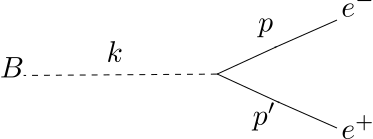
\includegraphics[scale=0.6]{Btoee} %noinstiki
  \caption{Feynman diagrams for $B\to e^+ e^-$} %noinstiki
  \label{fig:btoee} %noinstiki
\end{figure} %noinstiki
Let us define the one--particle states as in eq.~\eqref{eq:38}

\begin{align}
  | B(\mathbf{p})\rangle\equiv\sqrt{\frac{1}{V}}a^\dagger_{\mathbf{p}}|0\rangle 
\end{align}
 
\begin{align}
   | e^-(\mathbf{p},s)\rangle\equiv&\sqrt{\frac{1}{V}}f^\dagger_s(\mathbf{p})|0\rangle\nonumber\\
   | e^+(\mathbf{p},s)\rangle\equiv&\sqrt{\frac{1}{V}}\hat{f}^\dagger_s(\mathbf{p})|0\rangle\,, 
\end{align}
Using the commutation relations, our states are then normalized as
\begin{align}
\langle B(\mathbf{p})| B(\mathbf{p}')\rangle=&\frac{(2\pi)^3}{V}\delta^3(\mathbf{p}-\mathbf{p}')\nonumber\\
\langle e^-(\mathbf{p},s)| e^-(\mathbf{p}',s')\rangle=&\frac{(2\pi)^3}{V}\delta_{s s'}\delta^3(\mathbf{p}-\mathbf{p}')\nonumber\\
\langle e^+(\mathbf{p},s)| e^+(\mathbf{p}',s')\rangle=&\frac{(2\pi)^3}{V}\delta_{s s'}\delta^3(\mathbf{p}-\mathbf{p}')
\end{align}
As established in Sec.~\ref{sec:fock-space-real}, it is convenient to work in the discrete limit where \eqref{eq:26}
\begin{align}
   \delta^3(\mathbf{0})=\frac{V}{(2\pi)^3}\,.
\end{align}

Now we can write down the action of various field operators on different one particles states. 
Using the Fourier decomposition  of the scalar field in eq.~\eqref{eq:37}, and taking into account that 
$a_{\mathbf{p}}|0\rangle=0$, we have
\begin{align}
\label{eq:98}
   \phi_+(x)|B(\mathbf{k})\rangle=&\int d^3p \frac{1}{(2\pi)^3\sqrt{2\omega_{p} }}
\widehat{a}_{p} e^{-i p\cdot x }
|B(\mathbf{k})\rangle\nonumber\\
=&\int d^3p \frac{1}{(2\pi)^3\sqrt{2\omega_{p}}}
\widehat{a}_\mathbf{p} e^{-i p\cdot x }
\frac{1}{\sqrt{V}}\, \widehat{a}^\dagger_{\mathbf{k}}|0\rangle\nonumber\\
  =&\int d^3p \frac{1}{(2\pi)^3\sqrt{2\omega_{p}V}} e^{-i p\cdot x }
\, [\widehat{a}_{\mathbf{p}},\widehat{a}^\dagger_{\mathbf{k}}]|0\rangle\,.
\end{align}
%check normalization!
By usinbg the commutation relations in eq.~\eqref{eq:32} we have

\begin{align}
\phi_+(x)|B(\mathbf{k})\rangle  
=&\int d^3p \frac{\delta^{(3)}(\mathbf{p}-\mathbf{k})}{\sqrt{2\omega_{p}V}}
 e^{-i p\cdot x }|0\rangle
\end{align}
\begin{align}
\phi_+(x)|B(\mathbf{k})\rangle  
=&\frac{1}{\sqrt{2\omega_{k}V}}e^{-i k\cdot x }|0\rangle
\end{align}
Similarly, we have


\begin{align}
  \label{eq:99}
  \phi_+(x)|B(\mathbf{k})\rangle=&\frac{1}{\sqrt{2 \omega_k V}}e^{-i k\cdot x}|0\rangle\nonumber\\
  \psi_+(x)|e^-(\mathbf{p},s)\rangle=&\frac{1}{\sqrt{2 E_p V}}u_s(\mathbf{p})e^{-i p\cdot x}|0\rangle\nonumber\\
  \overline{\psi}_+(x)|e^+(\mathbf{p}',s')\rangle=&\frac{1}{\sqrt{2 E_{p'} V}}\bar{v}_{s'}(\mathbf{p}')e^{-i p'\cdot x}|0\rangle\,,
\end{align}

where $\omega_k$ and $E_p$ represent the energies of the scalar and the electron for the 3-momenta in the subscripts.

Similarly, for the adjoint operators
\begin{align}
  \label{eq:100}
   \langle B(\mathbf{k})|\phi_-(x)=&\langle0|\frac{1}{\sqrt{2 \omega_k V}}e^{i k\cdot x}\nonumber\\
  \langle e^-(\mathbf{p},s)|\overline{\psi}_-(x)=&\langle0|\frac{1}{\sqrt{2 E_p V}}\bar{u}_s(\mathbf{p})e^{i p\cdot x}\nonumber\\
  \langle e^+(\mathbf{p}',s')|\psi_-(x)=&\langle0|\frac{1}{\sqrt{2 E_{p'} V}}v_{s'}(\mathbf{p}')e^{i p'\cdot x}\,,
\end{align}
In the lowest order the only term which contributes to the matrix element is the term shown in Eq.~\eqref{eq:97}
The matrix element at first order in Eq.~\eqref{eq:96}, between the initial and the final state is then
\begin{align}
  S_{fi}^{(1)}=-i h \int d^4x\left\langle e^-(p)e^+(p')\left|\overline{\psi}_-\psi_-\phi_+\right|B(k)\right\rangle\,.
\end{align}
Using Eqs.~\eqref{eq:99}\eqref{eq:100}, we obtain
\begin{align}
  S_{fi}^{(1)}=&(-i h)\bar{u}_s(\mathbf{p}) v_{s'}(\mathbf{p}')
\int d^4x\,e^{i(p+p'-k)\cdot x}\frac{1}{\sqrt{2\omega_k V}}\frac{1}{\sqrt{2E_p V}}\frac{1}{\sqrt{2E_{p'} V}}\,.
\end{align}
Since
\begin{align}
  \int d^4x\,e^{i(p+p'-k)\cdot x}=(2\pi)^4\delta^4(k-p-p')\,,
\end{align}
we obtain
\begin{align}
  S_{fi}^{(1)}=&\left[\frac{1}{\sqrt{2\omega_k V}}\frac{1}{\sqrt{2E_p V}}\frac{1}{\sqrt{2E_{p'} V}}\right]
(2\pi)^4\delta^4(k-p-p')\left[(-i h)\bar{u}_s(\mathbf{p}) v_{s'}(\mathbf{p}')\right]
\end{align}
Comparing with Eq.~\eqref{eq:46} we have therefore that the relativistic matrix element is
\begin{align}
  i\mathcal{M}_{fi}=(-i h)\bar{u}_s(\mathbf{p}) v_{s'}(\mathbf{p}')\,,
\end{align}
and everything else is the history presented in Chapter~\ref{cha:two-body-decays}. 

\section{Wick Theorem}
\label{sec:wick-theorem}
From \cite{Lahiri:2005sm}. The normal ordering procedure involved putting all the annihilation operators to the right of all creation operators so that it annihilates the vacuum 

\section{Scattering}
\label{sec:scattering}
From the previous calculation we have
\begin{align}
S^{(n)}=  \frac{(-i)^n}{n!}\int\cdots\int d^4x_1 d^4x_2\ldots d^4x_n\,\operatorname{T}\{\mathcal{H}_I(x_1)\mathcal{H}_I(x_2)\ldots\mathcal{H}_I(x_n)\}\,.
\end{align}
The relevant term for the scattering
\begin{align}
  e^{-}(p_1)+e^{-}(p_2)\to   e^{-}(p_1')+e^{-}(p_2')
\end{align}
is
\begin{align}
S^{(2)}=&  \frac{(-i)^2}{2!}\int\int d^4x_1 d^4x_2\,\operatorname{T}\{\mathcal{H}_I(x_1)\mathcal{H}_I(x_2)\}\nonumber\\
=&  \frac{(-ih)^2}{2!}\int\int d^4x_1 d^4x_2\,\operatorname{T}\{:(\overline{\psi}\psi\phi)_{x_1}(\overline{\psi}\psi\phi)_{x_2}\}\nonumber\\
\supset& 
 \frac{(-ih)^2}{2!}\int\int d^4x_1 d^4x_2\,:(\overline{\psi}
\bcontraction{\psi}{\phi}{)_{x_1}(\overline{\psi}\psi}{\phi}
\psi\phi)_{x_1}(\overline{\psi}\psi\phi
)_{x_2}:\nonumber\\
=&\frac{(-ih)^2}{2!}\int\int d^4x_1 d^4x_2
\bcontraction{\,}{\phi}{(x_1)}{\phi}
\,\phi(x_1)\phi(x_2):(\overline{\psi}\psi)_{x_1}(\overline{\psi}\psi)_{x_2}:
\end{align}
The Wick contraction can be written as:
\begin{align}
  \bcontraction{\,}{\phi}{(x_1)}{\phi}
\,\phi(x_1)\phi(x_2)=&\langle0|T\{\phi(x_1)\phi(x_2)\}|0\rangle\nonumber\\
=&i\Delta_F(x_1-x_2)
\end{align}
while the non-zero contribution from the fermion product is
\begin{align}
  :(\overline{\psi}\psi)_{x_1}(\overline{\psi}\psi)_{x_2}:=&
:\overline{\psi}^\alpha(x_1)\psi^\alpha(x_1)\overline{\psi}^\beta(x_2)\psi^\beta(x_2):\nonumber\\
=&\overline{\psi}^\alpha_-(x_1)\overline{\psi}^\beta_-(x_2)\psi^\alpha_+(x_1)\psi^\beta_+(x_2)\,.
\end{align}
The $S$--matrix element the reads
\begin{align}
  S^{(2)}_{fi}=&\frac{(-ih)^2}{2}\int\int d^4x_1 d^4x_2\langle e^-(\mathbf{p}_1')e^-(\mathbf{p}_2')|
i\Delta_F(x_1-x_2)\overline{\psi}^\alpha_-(x_1)\overline{\psi}^\beta_-(x_2)\psi^\alpha_+(x_1)\psi^\beta_+(x_2)|e^-(\mathbf{p}_1)e^-(\mathbf{p}_2)\rangle\nonumber\\
=&\frac{(-ih)^2}{2}\int\int d^4x_1 d^4x_2\,i\Delta_F(x_1-x_2)\langle e^-(\mathbf{p}_1')e^-(\mathbf{p}_2')|
\overline{\psi}^\alpha_-(x_1)\overline{\psi}^\beta_-(x_2)\psi^\alpha_+(x_1)\psi^\beta_+(x_2)|e^-(\mathbf{p}_1)e^-(\mathbf{p}_2)\rangle\nonumber\\
=&\frac{(-ih)^2}{2}\int\int d^4x_1 d^4x_2\int\frac{d^4q}{(2\pi)^4}\,i\Delta_F(q)e^{i q\cdot(x_1-x_2)}\nonumber\\
&\times\langle e^-(\mathbf{p}_1')e^-(\mathbf{p}_2')|
\overline{\psi}^\alpha_-(x_1)\overline{\psi}^\beta_-(x_2)\psi^\alpha_+(x_1)\psi^\beta_+(x_2)|e^-(\mathbf{p}_1)e^-(\mathbf{p}_2)\rangle
\end{align}
The two particle Fock state is, after proper normalization
\begin{align}
  |e^-(\mathbf{p}_1)e^-(\mathbf{p}_2)\rangle=&\frac{1}{\sqrt{V}}f^\dagger(\mathbf{p}_2)f^\dagger(\mathbf{p}_1)|0\rangle
\end{align}
Therefore
\begin{align}
  \psi^\alpha_+(x_1)\psi^\beta_+(x_2)|e^-(\mathbf{p}_1)e^-(\mathbf{p}_2)\rangle=&
\int\frac{d^3k}{\sqrt{2E_k V}}\int\frac{d^3k}{\sqrt{2E_{k'}V}}
u^\alpha(\mathbf{k})u^\beta(\mathbf{k}')e^{-i k\cdot x_1}e^{-i k'\cdot x_2}\nonumber\\
&\times f(\mathbf{k})f(\mathbf{k}')f(\mathbf{p}_2)f(\mathbf{p}_1)|0\rangle
\end{align}

\begin{align}
  \psi^\alpha_+(x_1)\psi^\beta_+(x_2)|e^-(\mathbf{p}_1)e^-(\mathbf{p}_2)\rangle=&\frac{1}{\sqrt{2E_{p_1} V}}\frac{1}{\sqrt{2E_{p_2}V}}\nonumber\\
&\times\left[u^\alpha(\mathbf{p}_1)u^\beta(\mathbf{p}_2)e^{-i p_1\cdot x_1}e^{-i p_2\cdot x_2}
-u^\alpha(\mathbf{p}_2)u^\beta(\mathbf{p}_1)e^{-i p_2\cdot x_1}e^{-i p_1\cdot x_2}\right]|0\rangle
\end{align}
Following similar steps, we find
\begin{align}
  \langle e^-(\mathbf{p}_1')e^-(\mathbf{p}_2')|
\overline{\psi}^\alpha_-(x_1)\overline{\psi}^\beta_-(x_2)=&
\frac{1}{\sqrt{2E_{p_1}' V}}\frac{1}{\sqrt{2E_{p_2}'V}}\nonumber\\
&\times\langle0|\left[\bar{u}^\alpha(\mathbf{p}_1')\bar{u}^\beta(\mathbf{p}_2')e^{-i p_1'\cdot x_1}e^{-i p_2'\cdot x_2}
-\bar{u}^\alpha(\mathbf{p}_2')u^\beta(\mathbf{p}_1')e^{-i p_2'\cdot x_1}e^{-i p_1'\cdot x_2}\right]
\end{align}
As expected, the final result can be written in term of three different factors: the momentum conservation, normalization, and the relativistic amplitude
\begin{align}
  S^{(2)}_{fi}=i(2\pi)^4\delta^{4}\left(\sum_{i=1,2} p_i-\sum_{f=1,2}p'_f\right)
  \prod_{i=1,2}\frac{1}{\sqrt{2E_i V}}\prod_{f=1,2}\frac{1}{\sqrt{2E_f' V}}\mathcal{M}_{fi}
\end{align}
where
\begin{align}
  \mathcal{M}_{fi}=(ih)^2\left[
\bar{u}^\alpha(\mathbf{p}_2')\bar{u}^\beta(\mathbf{p}_1')\Delta_F(p_1-p_2')u^\alpha(\mathbf{p}_1)u^\beta(\mathbf{p}_2)
-\bar{u}^\alpha(\mathbf{p}_1')\bar{u}^\beta(\mathbf{p}_2')\Delta_F(p_1-p_1')u^\alpha(\mathbf{p}_1)u^\beta(\mathbf{p}_2)
\right]
\end{align}
The two contributions are displayed in Fig.~\ref{fig:sct}
\begin{figure} %noinstiki
  \centering %noinstiki
\includegraphics{scattering} %noinstiki
 \includegraphics{scattering2} %noinstiki
  \caption{fermion scattering} %noinstiki
  \label{fig:sct} %noinstiki
\end{figure} %noinstiki
Since
\begin{align}
  \Delta_F(q)=\frac{1}{q^2-m^2}
\end{align}
In the limit $q^2\ll m^2$
\begin{align}
  \Delta_F=-\frac{1}{m^2}
\end{align}
\begin{align}
  \mathcal{M}_{fi}=&\frac{h^2}{m^2}\left[
\bar{u}^\alpha(\mathbf{p}_2')u^\alpha(\mathbf{p}_1)\bar{u}^\beta(\mathbf{p}_1')u^\beta(\mathbf{p}_2)
-\bar{u}^\alpha(\mathbf{p}_1')u^\alpha(\mathbf{p}_1)\bar{u}^\beta(\mathbf{p}_2')u^\beta(\mathbf{p}_2)
\right]\nonumber\\
=&\frac{h^2}{m^2}\left[
\bar{u}(\mathbf{p}_2')u(\mathbf{p}_1)\bar{u}(\mathbf{p}_1')u(\mathbf{p}_2)
-\bar{u}(\mathbf{p}_1')u(\mathbf{p}_1)\bar{u}(\mathbf{p}_2')u(\mathbf{p}_2)
\right]
\end{align}
For one interaction of type $\overline{\psi}\Gamma\psi$ we should have
\begin{align}
  \mathcal{M}_{fi}=\frac{h^2}{m^2}\left[
\bar{u}(\mathbf{p}_2')\Gamma u(\mathbf{p}_1)\bar{u}(\mathbf{p}_1')\Gamma u(\mathbf{p}_2)
-\bar{u}(\mathbf{p}_1')\Gamma u(\mathbf{p}_1)\bar{u}(\mathbf{p}_2')\Gamma u(\mathbf{p}_2)
\right]
\end{align}
For the process 
\begin{align}
  e^-(p)+\nu_\mu(k)\to\mu^-(p')+\nu_e(k')
\end{align}
After the replacement $G_F/\sqrt{2}\equiv h^2/m^2$, we have
\begin{align}
  \label{eq:101}
  S^{(2)}_{fi}=i(2\pi)^4\delta^{4}\left(p_1+p_2-p'_1-p'_2\right)
  \frac{1}{\sqrt{2E_1 V}}\frac{1}{\sqrt{2E_2 V}}
  \frac{1}{\sqrt{2E_1' V}}\frac{1}{\sqrt{2E_2' V}}
  \mathcal{M}_{fi}
\end{align}
where
\begin{align}
  \mathcal{M}_{fi}=\frac{G_F}{\sqrt{2}}
\bar{u}_{\nu_e}(\mathbf{p}'_2)\Gamma u_e(\mathbf{p}_1)\bar{u}_\mu(\mathbf{p}'_1)\Gamma u_{\nu_\mu}(\mathbf{p_2})
\end{align}
The corresponding Feynman diagram is shown in Fig.~\ref{fig:sw}
\begin{figure} %noinstiki
  \centering %noinstiki
  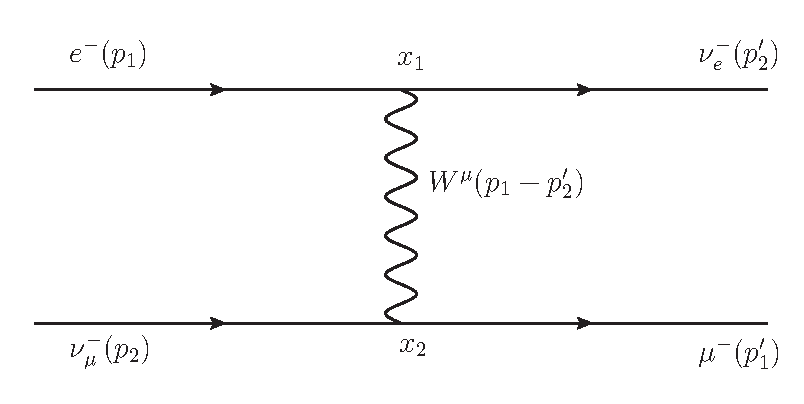
\includegraphics{scatteringw} %noinstiki
  \caption{scattering with four fermions} %noinstiki
  \label{fig:sw} %noinstiki
\end{figure} %noinstiki
From the standard model Lagrangian \cite{lsm}, we know that
\begin{align}
  \Gamma=\gamma^\mu(1-\gamma_5)
\end{align}
For $p\ll M_W^2$ the analysis is similar to the previous one with
\begin{align}
   \bcontraction{\,}{W^\mu}{(x_1)}{W^\nu}
\,W^\mu(x_1)W^\nu(x_2)=&\langle0|T\{W^\mu(x_1)W^\nu(x_2)\}|0\rangle\nonumber\\
\approx&\int\frac{d^4q}{(2\pi)^4}\frac{g^{\mu\nu}}{M_W^2}e^{-i q\cdot(x_1-x_2)}
\end{align}
Therefore we have

\begin{align}
  \mathcal{M}_{fi}=\frac{G_F}{\sqrt{2}}
\bar{u}_{\nu_e}(\mathbf{p}_2')\gamma^\mu(1-\gamma_5)u_e(\mathbf{p_1})
\bar{u}_\mu(\mathbf{p}_1')\gamma_\mu(1-\gamma_5)u_{\nu_\mu}(\mathbf{p_2})
\end{align}
We now must sqaure the scattering amplitude, $\mathcal{M}$, and summing up over final spin states, and averaging over the intial spin states, as we did in Eq.~\eqref{eq:81}
\begin{align}
  \label{eq:102}
  \overline{|\mathcal{M}|^2}=64\,G_F^2\,(p_1\cdot p_2)(p_1'\cdot p_2')
\end{align}

From Eq.~\eqref{eq:74}
\begin{align}
  \label{eq:103}
  \frac{d\sigma}{d\Omega}=\frac{1}{64\pi^2s}\left(\frac{s-m_\mu^2}{s-m_e^2}\right)\overline{|\mathcal{M}|^2}
\end{align}

The center of mass (CM) frame is defined by the condition in Eq.~\eqref{eq:55}:
\begin{align}
  \mathbf{p}_1+\mathbf{p}_2=0
\end{align}
The $\delta$--function in Eq.~\eqref{eq:101}
\begin{align}
  \delta^{(4)}(p_1+p_2-p_1'-p_2')=\delta^{(3)}(\mathbf{p}_1+\mathbf{p}_2-\mathbf{p}_1'-\mathbf{p}_2')
\delta(E_1+E_2-E_1'-E_2')
\end{align}

implies
\begin{align}
  \mathbf{p}_1+\mathbf{p}_2-\mathbf{p}_1'-\mathbf{p}_2'=0 \overset{\text{CM}}{\Rightarrow}
  \begin{cases}
    \mathbf{p}_1=-\mathbf{p}_2\\
    \mathbf{p}_1'=-\mathbf{p}_2'\\
  \end{cases}
\end{align}
Moreover
\begin{align}
  \sqrt{s}=E_1+E_2
\end{align}
In the CM frame
\begin{align}
\label{eq:104}
s=&\left(E_1+E_2\right)^2\nonumber\\
=&\left(\sqrt{\mathbf{p}_1^2+m_1^2}+\sqrt{\mathbf{p}_2^2+m_2^2}\right)^2\nonumber\\
=&\left(\sqrt{\mathbf{p}_1^2+m_e^2}+\sqrt{\mathbf{p}_1^2+m_{\nu_e}^2}\right)^2
\end{align}
Therefore
\begin{align}
  \label{eq:105}
  E_2=|\mathbf{p}_1|
\end{align}
In this case
\begin{align}
  \label{eq:106}
  s=&\left(\sqrt{\mathbf{p}_1^2+m_e^2}+|\mathbf{p}_1|\right)^2
\end{align}
\begin{align}
   \sqrt{s}=&\sqrt{\mathbf{p}^2_1+m_e^2}+|\mathbf{p}_1|
\end{align}
\begin{align}
\left(\sqrt{s}-|\mathbf{p}_1|\right)^2=&\mathbf{p}^2_1+m_e^2\nonumber\\
s-2\sqrt{s}\mathbf{p}_1+\mathbf{p}^2_1=&\mathbf{p}^2_1+m_e^2\nonumber\\
s-2\sqrt{s}\mathbf{p}_1=&m_e^2
\end{align}
\begin{align}
  |\mathbf{p}_1|=\frac{s-m_e^2}{2\sqrt{s}}
\end{align}
From Eq.~\eqref{eq:105} we have
\begin{align}
  \sqrt{s}=&E_1+E_2\nonumber\\
  =&E_1+|\mathbf{p}_1|
\end{align}
\begin{align}
  E_1=&\sqrt{s}-|\mathbf{p}_1|\nonumber\\
  =&\sqrt{s}+\frac{-s+m_e^2}{2\sqrt{s}}\nonumber\\
  =&\frac{2s-s+m_e^2}{2\sqrt{s}}\nonumber\\
  =&\frac{s+m_e^2}{2\sqrt{s}}
\end{align}
Then, by using again eq.~\eqref{eq:105}:
\begin{align}
  p_1\cdot p_2=&E_1E_2-\mathbf{p}_1\cdot\mathbf{p}_2\nonumber\\
  =&E_1|\mathbf{p}_1|+\mathbf{p}_1^2\nonumber\\
=&\frac{(s-m_e^2)(s+m_e^2)}{4s}+\frac{(s-m_e^2)^2}{4s}\nonumber\\
=&\frac{(s-m_e^2)}{4s}(s+m_e^2+s-m_e^2)\nonumber\\
=&\frac{1}{2}(s-m_e^2) 
\end{align}
As $p_2^2={p_2'}^2=0$, we have from $\delta$--function
\begin{align}
  (p_1+p_2)^2=&(p_1'+p_2')^2\nonumber\\
  (p_1+p_2)^2=&(p_1'+p_2')^2\nonumber\\
  p_1^2+2p_1\cdot p_2+p_2^2=&{p_1'}^2+2p_1'\cdot p_2'+{p_2'}^2\nonumber\\
  p_1^2+2p_1\cdot p_2=&{p_1'}^2+2p_1'\cdot p_2'\nonumber\\
  m_e^2+2p_1\cdot p_2=&m_\mu^2+2p_1'\cdot p_2'
\end{align}
\begin{align}
  p_1'\cdot p_2'=p_1\cdot p_2-\frac{1}{2}(m_\mu^2-m_e^2)
\end{align}
\begin{align}
  p_1'\cdot p_2'=\frac{1}{2}(s-m_\mu^2) 
\end{align}
Replacing back in Eq.~\eqref{eq:102} and then in Eq.~\eqref{eq:103} we have
\begin{align}
  \frac{d\sigma}{d\Omega}=\frac{1}{64\pi^2s}\left(\frac{s-m_\mu^2}{s-m_e^2}\right)
64G_F^2\frac{1}{2}(s-m_e^2)\frac{1}{2}(s-m_\mu^2)
\end{align} 
\begin{align}
    \frac{d\sigma}{d\Omega}=\frac{G_F^2}{4\pi^2}\frac{(s-m_\mu^2)^2}{s}
\end{align}
\begin{align}
\sigma  =\frac{G_F^2}{\pi}\frac{(s-m_\mu^2)^2}{s}
\end{align}
Note that $\sigma\propto s$.
%\left(\right)
%\left[\right]


%%% Local Variables: 
%%% mode: latex
%%% TeX-master: "beyond"
%%% End: 
